\documentclass{article}

\usepackage{hyperref}
\usepackage{parskip}
\usepackage{amsthm}
\usepackage{amsmath}
\usepackage{amssymb}
\usepackage{wrapfig}
\usepackage{graphicx}
\usepackage{listings}
\usepackage{color}
\usepackage{fullpage}
\newcommand{\code}{\texttt}

\author{Micah Wylde\\Jeffrey Ruberg}
\date{\today}
\title{Autonomous Agents:\\
A Hybrid Dynamical System for Vehicle Navigation\\
Comp 352}

\begin{document}
\maketitle

\section{Introduction}
Self-driving cars hold much promise for saving fuel, time and
lives. Human-driven vehicles are responsible for millions of traffic accidents
and over 30,000 deaths annually in the US alone. Humans can also make poor
decisions in regards to routes, leading to traffic jams and wasted fuel. Safe,
effective autonomous cars could largely solve these issues. AI researchers have
been interested in the potential for vehicular navigation since the 1960s. In
order to spur development in this area, the Defense Advanced Research Projects
Agency (DARPA) organized the Grand Challenge in 2004, which tasked contestants
to build cars which could autonomously navigate a 142 mile-long course in the
Mojave desert. Though none of the vehicles could finish the course, a second
competition the next year was more successful. Four teams finished in the
allotted time, traversing a treacherous 132 mile desert course with no human
guidance. Building on this achievement, in 2007 DARPA organized the Urban
Challenge which took place in a simulated suburban environment. To win, cars had
to navigate a maze of streets while accounting for other traffic and following
California traffic laws at all times. Six teams finished the 61 mile course with
the winner, ``Boss'' from CMU, taking a little more than four hours
\cite{robotic_cars}.

There are many challenges involved in autonomous driving and robot navigation in
general. In the real world one must deal with unreliable and imperfect sensor
data, imprecise localization technologies and other perception issues. Even in
simulation the challenges of successful navigation are immense. Cars must follow
traffic laws, get to their destination quickly and efficiently and act safely at
all times, even in unexpected situations. As far as the actual navigation, there
are two general approaches: deliberative and reactive. As an example of the
former, $A^*$ is an efficient and optimal graph search algorithm which is very
effective at finding the best route between two points but cannot handle the
dynamism of the real world. Dynamical systems-based navigation is a reactive
strategy that uses force fields to guide agents away from obstacles and towards
their target. However, it is purely local and has trouble finding optimal paths
to distant goals. In this paper we present simulated agents which use each
technique as well as a hybrid agent which makes use of $A^*$ for global
navigation and dynamical systems for local navigation.


\section{Methods}

To create an autonomous agent that navigates while simulating a car's behavior
and traffic laws, we took three general approaches: deliberative planning
through $A^*$ search, reactive navigation through a dynamical system, and a
hybrid of deliberative planning and reactive motion. The system architecture
consists of a server and a separate client for each agent. Our goal
was to produce agents which could navigate in a realistic environment
while following traffic laws and acting safely at all times even when
faced with dynamic, unexpected obstacles like pedestrians and other
cars. Due to the great difficulty of producing the simulation, we were
forced to scale back our ambitions to merely simulating driving in a
relatively static world.

\subsection{System Architecture}

The project is written in Ruby, specifically JRuby\footnote{JRuby is
  an implementation of the Ruby Programming Language on top of the
  Java Virtual Machine, which allows integration between Java and Ruby
  code} to utilize Java2D for the graphical display. As a result, the
server code runs solely under JRuby, but client code can additionally
be run using Ruby 1.9. Agents are represented both on the client and
server end; server agents perform motion and display-related
calculations, and client agents contain all the navigation inference
and decision-making and ultimately send decisions (restricted to
behavior variables) back to the server again. Agents communicate with
the server over sockets by serializing hashes with YAML\footnote{YAML
  (a recursive acronym for YAML Ain't Markup Language) is a
  language-independent data serialization standard which allows easy
  conversion of data structures to and from a string
  representation.}. Every part of the simulation is asynchronous: the
display is constantly rendering the current state of the world as
quickly as it can. The server agents are constantly recalculating
their state variables according to their velocity and amount of
turning ($\delta$). The message loop is as follows: the client agents,
which actually do the navigation computations, receive messages from
the server with their current states. They then process that according
to their operation and decide on an action, which is then sent to the
server. The server carries out the action in the environment and sends
the new state variables back to the agent.

\begin{figure}[h]
  \begin{center}
    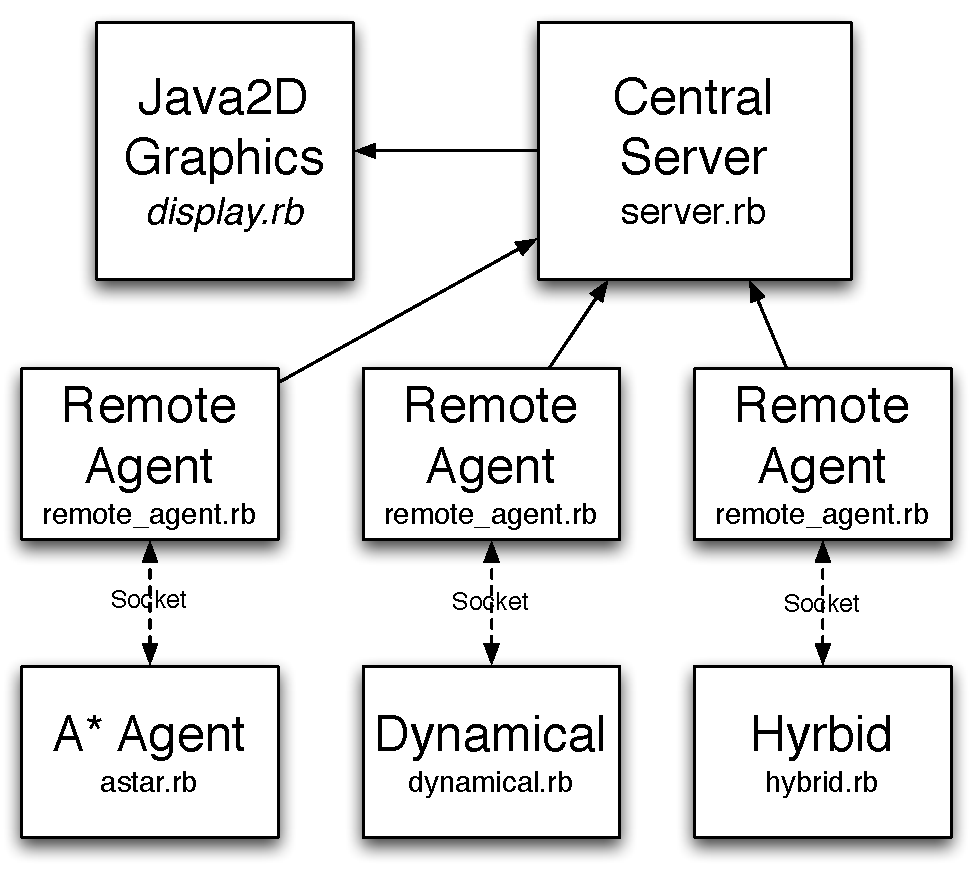
\includegraphics[width=0.5\textwidth]{architecture}
  \end{center}
  \caption{The system architecture of the simulation. Solid lines connect
    components included in the same process, while dotted lines indicated socket
    connections between discrete processes.}
  \label{architecture}
\end{figure}

The simulation is composed of many source files which control various
pieces. The general architecture is given in figure
\ref{architecture}, while the roles of the individual files are listed
below. More information can be found in the documentation in each class.

\begin{description}
\item[app.rb] The point of entry for the program. Processes
  command-line options and can optionally start a server, start a new
  agent, or run tests.

\item[client\_agent.rb] Contains the \code{ClientAgent} class, the
  super class which every client agent inherits. Client agents receive
  messages from remote server agents, process the message (based on
  their form of navigation), and then send back a response in their
  behavior variable space.

\item[constants.rb] Contains various general constants that may be
  used in several locations or files, or that may be particularly useful to
  tweak with.

\item[display.rb] Contains all of the display code used to generate
  our rendering of the world.

\item[map.rb] Contains the classes, specifically \code{Map}, which
  encode information provided from real map data.

\item[pqueue.rb] A priority queue implementation used for $A^*$ search.

\item[remote\_agent.rb] Contains the \code{RemoteServerAgent} class,
  which is a subclass of \code{ServerAgent}. Essentially, a remote
  server agent is a server agent which is tied to a specific client
  agent and communicates with that client agent.

\item[server\_agent.rb] Contains the \code{ServerAgent} class, which
  contains all the base representation and calculations needed for an agent (for
  example, the server agent computes various points needed to display the agent
  graphically).

\item[server.rb] Contains the socket server which handles agent connections.

\item[socket.rb] Contains code for handling communication between
  clients and the server

\item[util.rb] Contains a collection of geometry classes
  (\code{Point}, \code{Vector}, etc.) which are useful in the display
  and other various places (most notably in dynamical navigation
  calculations).

\item[agents/astar.rb] Contains a client agent that deliberatively
  plans paths using $A^*$ search.

\item[agents/dynamical.rb] Contains a client agent that navigates
  through a purely dynamical system-based approach.

\item[agents/hybrid.rb] Contains a client agent that navigates through
  a combination of deliberative planning and dynamical systems.

\item[agents/simple.rb] Contains a very primitive client agent (that
  can hardly be called an agent) which allows us to easily test the
  motion calculations performed by server agents.

\end{description}

\subsection{Simulation}
To provide a realistic environment for navigation tests, we used
real-world map data from OpenStreetMap.org, which provides
XML-formatted maps for the entire world. The data format, called OSM,
provides a graph representation of a road system; streets are
represented by placing nodes wherever the road turns or intersects
other roads, with edges connecting each node. To provide testing data,
we used the website to export maps of Hayward, CA and Santa Cruz,
CA. We wrote a program, \code{osm\_convert}, which converts an OSM XML
file to a YAML format. In \code{map.rb} we then read this YAML data
and construct an internal representation of the graph, converting
points specified by latitude and longitude to a scale of meters.

In order to construct a simulation from this data, we needed to make
roads from the edges of the graph. We did so by finding the normal
vector to the edge and computing line segments that were a constant
ROAD\_DIST from the center-line. With the four corners, we could then
draw the roads as polygons as well as use them for purposes of
obstacle avoidance as described below. However, the naive
implementation of this algorithm produced some overlapping walls and
some walls which were too short. We therefore employ a clipping
algorithm which ensures that the road edges meet smoothly. This does,
however, leave empty spaces at intersections which appear green in the
display.

The simulation has been designed for realism, with the agents
responding in a physically plausible way according to two state
variables which the agents can set: acceleration and $\delta$, the
amount that the wheel is turned. Raising $\delta$ above 0 causes the
wheels to turn right and the car to follow in a circle, while lowering
it below 0 causes the wheels to turn left. In this way we hope to
demonstrate a direct analogy to control of robotic cars, which
primarily concerns the acceleration/brake and steering. However
we had difficulty producing working navigation with this scheme, so
the agents described below work by setting $\phi$, the heading angle,
directly.


\subsection{Deliberative Agent}
\begin{figure}[h]
  \begin{center}
    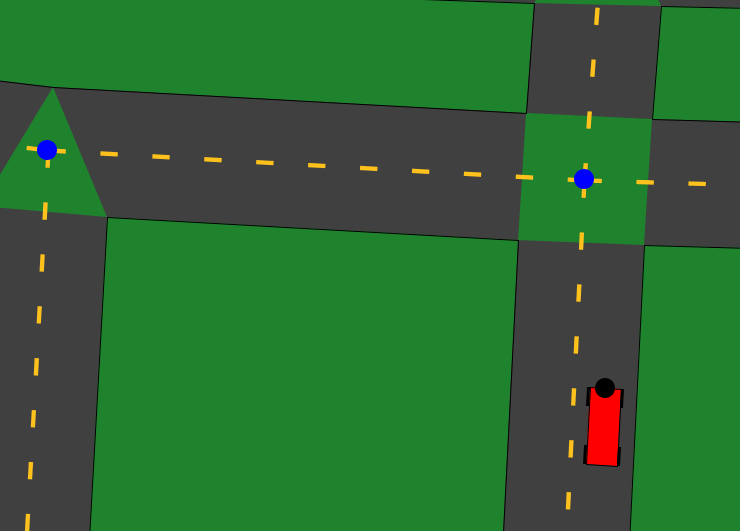
\includegraphics[width=0.5\textwidth]{astar}
  \end{center}
  \caption{$A^*$ navigation at work. The blue dots indicate the route.}
  \label{astar}
\end{figure}
We do deliberative navigation using the $A^*$ graph search algorithm,
which takes a heuristic function $h$ and finds a path between two
nodes on a graph. If $h$ satisfies certain properties, the path
returned will be optimal. We use the Euclidean distance formula
$h(n_1, n_2)=\sqrt{(n_1.x - n_2.x)^2 + (n_1.y - n_2.y)^2}$ which
satisfies these properties. The agent is modeled as a finite state
machine with four states: start, straight, turn, and replan. The agent
begins operation in the start state wherein it calculates the optimal
route to its destination. Once that is done, it begins traveling
forward until it is twice the road width from its starting node. It
then transitions to straight mode, where it ensures that its $\phi$ is
set parallel to the road. When it reaches a node, it pops the top node
off the route stack and enters turn mode. In turn mode it sets its
$\phi$ parallel to the vector between its target node (the node on the
top of the route stack) and itself. This ensures the agent stays on
the road at all times. Finally, when the agent has traveled past the
node, it reverts back to straight mode. If the agent reaches a node
which is not the next on its route, it enters replan mode, where it
immediately stops and calculates a new route to its destination from
its current position. Replanning can also be triggered by the server
sending a new destination.

\subsection{Reactive Agent}
\begin{figure}[h]
  \begin{center}
    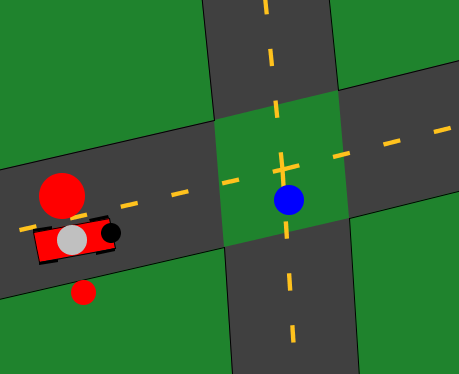
\includegraphics[width=0.5\textwidth]{dynamical}
  \end{center}
  \caption{Dynamical navigation at work. The red circles are obstacles
    that move along the road with the agent, while the blue circle is
    an intermediate target.}
  \label{dynamical}
\end{figure}

The reactive agent uses a dynamical systems approach for
navigation. It forces the agent to stay in its lane by placing
obstacles along the walls of the lane. We use a series of targets
place at the next intersection to guide the agent along the desired
path. The most interesting detail of our dynamical system is our
obstacle representation. The math of dynamical systems requires that
all objects in the world be represented as circles, which is a poor
fit for long straight obstacles such as walls. There are two
conventional solutions to representing non-circular obstacles: use one
large circle that bounds the obstacle or use many small circles along
the obstacle. The first is untenable for the narrow corridors a car
must pass through, while the second would require a very large number
of circles and the corresponding computation. Our approach is to use a
single circular obstacle per wall which follows the agent and which
grows in size as the agent gets closer. Implementing this requires
only basic geometry. We find the vector between the wall and the agent
perpendicular to the road and displace the center of the circle from
the road by a factor of the distance between the agent and the edge of
the road. 

Like the deliberative agent, the reactive agent is modeled
as a FSM with states start, normal, intersection and turn. Start
waits until the agent is properly set up and chooses the initial
target as the node the agent is currently facing, then transitions to
normal mode. When in normal mode, the agent navigates until it
reaches a node at which point it transitions to either intersection
mode if the node it's reached has more than one neighbor or turn mode
otherwise. If it's an intersection (which means more than one choice
of which way to go) the agent computes the set $T = \{t\;|\;t\neq
n_1,t \mbox{ is a neighbor of } n_0\}$ where $n_0$ is the node we've
arrived at and $n_1$ is the node we've left. It then finds the $t\in
T$ which minimizes $abs(u-v)$ where $u$ is the vector from the agent
to the destination and $v$ is the angle from $n_0$ to $t$. We're
trying to discover the best route using purely local information, so
we find the path that appears to take us in the correct direction.

We set our dynamical parameters somewhat arbitrarily as follows: $m =
2, d_0 = 0.1, a = 20, \sigma = 1, h_1 = 10$. We do not use weights as
we found them unnecessary. The most crucial parameter for our
simulation seems to be $a$, the target attractor scaling factor. Lower
$a$ values do not produce working navigation.

\subsection{Hybrid Agent}
The hybrid agent was designed with the understanding that vehicular
navigation is really a hybrid problem. Unlike more free-form
environments, road systems are very limiting to dynamical
navigation. Even though the agent may think its going in roughly the
right direction, it has no way of knowing from purely local
information whether it can even reach its destination by its
path. Methods like $A^*$ which look at global map data can solve this
issue by finding the best path to take from every intersection so that
the agent reaches the target in the minimum amount of time. However,
deliberative methods do not handle the moment-to-moment navigation
issues well, particularly in a dynamic environment. The best option
seems to be a combination of the two: a hybrid dynamical agent. This
agent behaves mostly like the dynamical agent described above except
for how target selection works. Instead of choosing the next target
using purely local information, we initially compute the $A^*$ route
as described in the deliberative section and use each node of that as
the intermediate targets.

\section{Results}

\section{Conclusion}
\subsection{Unreached goals}
- cached map rendering
- realistic choice variables

\end{document}
